\documentclass[a4paper, 12pt, twoside]{article}
\usepackage[utf8]{inputenc}		% LaTeX, comprend les accents !
\usepackage[T1]{fontenc}		
\usepackage[francais]{babel}
\usepackage{lmodern}
\usepackage{ae,aecompl}
\usepackage[top=2.5cm, bottom=2cm, 
			left=3cm, right=2.5cm,
			headheight=15pt]{geometry}
\usepackage{graphicx}
\usepackage{eso-pic}	
\usepackage{array}	
\makeatletter
\def\@ecole{école}
\newcommand{\ecole}[1]{
  \def\@ecole{#1}
}
\def\@domaine{}
\newcommand{\domaine}[1]{
  \def\@domaine{#1}
}

\def\@specialite{Spécialité}
\newcommand{\specialite}[1]{
  \def\@specialite{#1}
}


\def\@master{Master}
\newcommand{\master}[1]{
  \def\@master{#1}
}

\def\@adresse{Adresse}
\newcommand{\adresse}[1]{
  \def\@adresse{#1}
}

\def\@encadranta{}
\newcommand{\encadranta}[1]{
  \def\@encadranta{#1}
}

\def\@encadrantb{}
\newcommand{\encadrantb}[1]{
  \def\@encadrantb{#1}
}
\def\@auteura{}{}{}
\newcommand{\auteura}[1]{
  \def\@auteura{#1}
}
\def\@auteurb{}{}{}
\newcommand{\auteurb}[1]{
  \def\@auteurb{#1}
}
\def\@auteurc{}{}{}
\newcommand{\auteurc}[1]{
  \def\@auteurc{#1}
}
\def\@auteurd{}{}{}
\newcommand{\auteurd}[1]{
  \def\@auteurd{#1}
}
\makeatother




\makeatletter
\newcommand{\pagedegarde}{
\newgeometry{top=2.5cm, bottom=1cm, left=2cm, right=1cm}
  \begin{titlepage}
  \centering
      
\includegraphics[width=1\textwidth]{limogelogo.pdf}
    \vspace{1cm}
      {\huge 
    \vspace{0.5cm}
        {\huge\bfseries \@ecole}\\
    \vspace{0.2cm}
        {\Large\bfseries \@domaine}\\
    \vspace{0.5cm}
        {\Large\bfseries Master 1 }\\
    \vspace{0.2cm}
        {\large\bfseries Sécurité informatique et cryptologie }\\
    \vspace{1cm}
    	MEMOIRE DU SECOND SEMESTRE}\\
    \vfill
       {\LARGE \color[rgb]{0,0,1} \bfseries{\@title}} \\
    \vspace{2cm}
    	{\bfseries \@auteura}\\
    	{\bfseries \@auteurb}\\
    	{\bfseries \@auteurc}\\
    	{\bfseries \@auteurd}\\
    \vspace{0.5cm}
        Encadrants :\\
        {\bfseries \@encadranta}\\
        {\bfseries \@encadrantb}\\
    \vspace{0.5cm}
        {\Large\bfseries \@date}\\
    \vfill
  \end{titlepage}
\restoregeometry
}
\author{}
\auteura{Thanina \textsc{Alili}}
\auteurb{Thibault \textsc{Debonnière}}
\auteurc{Baptiste \textsc{Decrand}}
\auteurd{Ndiasse \textsc{Thioune}}
\title{Analyse Forensic d'un Ransomware}
\master{Master 1 Informatique}
\specialite{CRYPTIS}
\encadranta{Jean-Louis \textsc{Lanet}}
\encadrantb{Benoit \textsc{Crepin}}
\date{Decembre 2017}
\ecole{UNIVERSIT\'{E} DE LIMOGES}
\domaine{
	\textbf{FACULT\'{E} DES SCIENCES ET TECHNIQUES}
}
\begin{document}
\pagedegarde
\tableofcontents
\newpage
\section{Introduction}
\paragraph{}

Dans le cadre de la première année en Master informatique à l'université de Limoges, nous avions à réaliser un projet de développement logiciel. Ceci constitue le rapport de progression intermédiaire.

\paragraph{}
Ce sujet porte sur un outil d'Analyse Forensic de ransomware et a été proposé par M. JL Lanet. Le programme a pour fonction, à partir d'une base de donnée appelée "dictionnaire", de catégoriser un malware depuis une capture de l'image mémoire d'un système contaminé. Une fois classifié, ce dernier peut alors être traité et neutralisé de la bonne façon.

\paragraph{}
 Notre objectif à la date du 7 janvier était de pouvoir proposer un prototype fonctionnel sur un nombre restreint de métrique et un dictionnaire basique. Au second semestre cette base sera amené à être optimisée et complétée.

\paragraph{}
Le travail à pu être réparti par les métriques d'analyse que nous avons utilisé au nombre de 8 pour le moment où chacun a eu à étudier, rechercher les intérêts et défauts selon le cas de figure.




\newpage
\section{Rappel du principe d'un Ransomware}

\paragraph{}
Le Ransomware fait partie de la famille des malwares, c'est un logiciel malveillant apparu fin des années 80 qui est toujours d'actualité, on peut notamment citer le logiciel Wannacry qui a réussi à contaminer des grandes entreprises telles que Renault ou FedEx en mai 2017. Ces logiciels menacent l'utilisateur en bloquant l'accès aux données d'un système et obligent le propriétaire à payer une rançon afin d'espérer débloquer l'appareil infecté. Mais biensûr, rien ne garantie que les ravisseur remettent effectivement la clef de décryptage.(on estime à moins de 10\% le nombre de machine débloquées après paiement) 

\begin{figure}[h]
  \centering{
  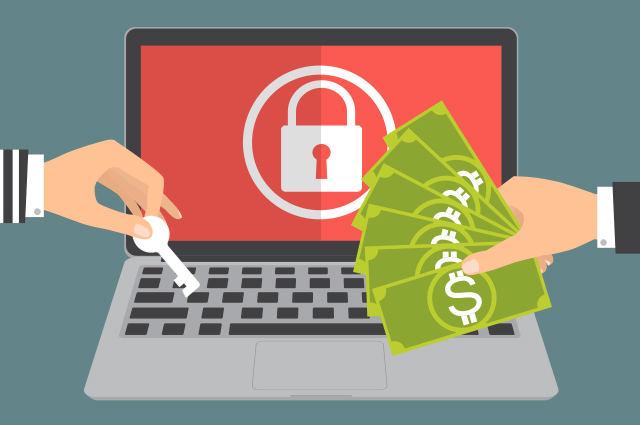
\includegraphics[scale=0.40]{Ransomware.jpg}}
\end{figure}

\paragraph{}
Il existe plusieurs types de ransomware, on peut les distinguer sur la manière qu'ils ont de chiffrer les données, en utilisant un chiffrement à clef asymétrique ou symétrique par exemple. Certains ransomwares ne chiffrent pas les données mais vont juste bloquer l'accès au système empêchant l'utilisateur peu expérimenté d'accéder à ces données. On peut aussi distinguer les ransomwares par le message de menace, en fonction du langage écrit ou bien de leurs contenus: certains sont des scarewares et se font passer pour des agences gouvernementales ou bien pour des antivirus.
\paragraph{}
Ces plans mémoires correspondent à un instant T de la mémoire, on peut alors récupérer plusieurs informations qui vont nous permettre de caractériser le ransomware tel que les noms d’API qui souhaite utiliser, les librairies (.dll) utilisées, la page de rançon voir même les clefs de chiffrage. Cependant ces informations peuvent être incomplètes ou indisponibles en fonction de quand la capture a été faite, ce qui fait que chaque plan mémoire est unique et qu’on ne pourra se reposer sur un simple algorithme de pattern matching et qu'il faudra utiliser des algorithmes approchés afin de calculer le taux de ressemblance avec les familles de malwares.
\newpage
\section{Application}
\subsection{Présentation détaillée}

\paragraph{}
L'application que nous allons créer devra donc permettre à l'utilisateur de lui fournir une capture mémoire d'un ransomware et de récupérer des résultats qui lui permettront de savoir à quelle classe ce ransomware appartient.

\paragraph{}
Cette application sera composée de trois modules.
La première s’occupera d’extraire les données du dump mémoire sous forme de chaîne de caractères et devra filtrer les informations illisibles et inutiles afin de ne récupérer que les appels systèmes, les librairies utilisés et des informations spécifiques.Pour notre premier prototype, les capture nous ont été fournies "pré-traitée" sous forme de liste de chaaine de caractère. Là commmence la première problèmatique, à savoir séparer les informations "utiles" des autres. Par exemple, sur les chaines de caractères récupérées nous pouvons retrouver plusieurs types : 

\begin{figure}[h]
    \begin{minipage}[c]{.46\linewidth}
        \centering
        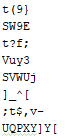
\includegraphics{Capture1.PNG}
        \caption{}
    \end{minipage}
    \hfill%
    \begin{minipage}[c]{.46\linewidth}
        \centering
        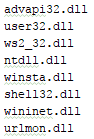
\includegraphics{Capture2.PNG}
        \caption{}
    \end{minipage}
\end{figure}

Ici, on remarquera que la figure 2 montre des lignes beaucoups plus intéressantes pour notre travail de classification. Pour ce premier semestre, notre filtrage reste encore limité mais pourra être étoffé par la suite(Par comparaison avec un "goodware" par exemple)


\paragraph{}

Une fois ces données récupérées, elles seront transformées en vecteurs binaires et seront soumises à huit métriques.Il s'agit ici de différentes formules qui irront comparer une à une les la présence des chaîne que nous avons récupérer à l'étape précédente. Nous obtiendront alors un poucentage de similarité entre elles. Ainsi les vecteur les plus proches pourront assimilé à un même groupe. Nous détailleront chaque métriques utilisés plus loin dans la partie dédiée.

\begin{figure}[h]
  \centering
  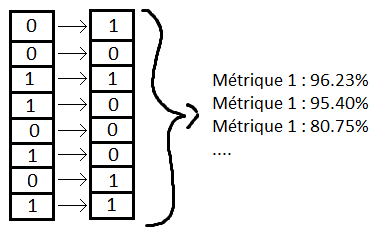
\includegraphics[scale=0.70]{Capture3.png}
  \caption{Schéma métrique}
\end{figure}




\paragraph{}
Le troisième module sera une interface graphique qui permettra de visualiser et de mettre en avant les résultats obtenus ainsi que les informations importantes du ransomware (famille du ransomware, page de rançon ou serveur associé, clé de chiffrage, etc.).










Pour réaliser ces comparaisons, nous avons à notre disposition grâce aux LHS de Rennes d'une base de données de plan mémoire (dump de binaires dépaquetés) de ransomware dont on connaît pour une partie à quelles classes ils appartiennent. Ces derniers serviront d'une base d'apprentissage afin de tester le bon fonctionnement de notre programme et la fiabilité des résultats obtenus.

\begin{figure}[h]
  \centering{
  
\includegraphics[scale=0.40]{Capture4}}
  \caption{INRIA Rennes}
\end{figure}


\subsection{Description des métriques étudiés}

\paragraph{}
Comme dit plus haut, nous utilisons pour la comparaison entre nos vecteurs, 8 métriques différents. Cette partie détaille le fonctionnement de chacun. Pour se faire, nous définissons le système suivant :

\paragraph{}
Une fonction de similitude renverra 0 si les deux vecteurs sont égaux et tendra vers l'infini la dissimilarité.Une fonction de distance renverra une valeur entre 0 et 1, 1 représentant l'égalité des deux vecteurs.
\paragraph{}
Un vecteur binaire sera construit de telle manière que la présence d'une chaîne de caractères d'un appel système ou d'une librairie sera représenté par un 1 et l'absence par un zéro.
\paragraph{}
Les vecteurs binaires de comparaison qui représenteront les familles de ransomware seront construit depuis une base de données contenant des captures mémoire de ransomware connu.
\paragraph{}
Soit A et B deux vecteurs binaires de taille $n$.

On définit:

   $n_{A0}$, la quantité de 0 du vecteur A.
   
   $n_{A1}$, la quantité de 1 du vecteur A.
    
   $S0_{A}0_{B}$, le nombre de couple (0,0) pour les vecteurs binaires X,Y quand $A_{i} = 0$ et $B_{i} = 0$.

   $S1_{A}0_{B}$, le nombre de couple (1,0) pour les vecteurs binaires X,Y quand $A_{i} = 1$ et $B_{i} = 0$.

   $S0_{A}1_{B}$, le nombre de couple (0,1) pour les vecteurs binaires X,Y quand $A_{i} = 0$ et $B_{i} = 1$.

   $S1_{A}1_{B}$, le nombre de couple (1,1) pour les vecteurs binaires X,Y quand $A_{i} = 1$ et $B_{i} = 1$.\\
   


\subsubsection{Similarité de Cosine}
Le calcul de la similarité de Cosine s'obtient par le rapport entre le produit scalaire et le produit de la norme des vecteurs.

\[
    S = \frac{A \cdot B}{||A|| \cdot ||B||}
    \Leftrightarrow S = \frac{\sum_{i=0}^n A_{i}B_{i}}{\sqrt{\sum_{i=0}^n A_{i}}\times\sqrt{\sum_{i=0}^n B_{i}}}
    \Leftrightarrow S = \frac{S1_{A}S1_{B}}{\sqrt{n_{A1}}\times \sqrt{n_{B1}}}
\]\\
Après cette simplification, on remarque que la similarité de Cosine se base uniquement sur la présence de chaîne de caractères, et constitue donc le rapport entre la présence commune de chaînes et le produit de la quantité de présence de chaque vecteurs.
\subsubsection{Distance de Hamming}
La distance de Hamming peut être définie comme un quantificateur capable de faire la différence entre deux séquences de symboles de même longueur.
Le principe de la distance de Hamming consiste à comparer les caractères les uns à la suite des autres.
Il faut calculer le nombre de bits qui sont différents entre deux vecteurs binaires, c’est à dire pour deux séquences de caractères x et y , on parcourt toutes les caractères de x et de y , puis on regarde si la valeur de x et de y sont identiques dans toutes les colonnes , si oui on divise le nombre de (x,y) similaires présent dans le vecteur avec la taille du vecteur N. 

On peut l’illustrer par la formule suivant:

\begin{equation}
   H = \frac{S1_{A}1_{B}+S0_{A}0_{B}}{S1_{A}1_{B} + S0_{A}1_{B}+S1_{A}0_{B} + S0_{A}0_{B}}
\end{equation}


\subsubsection{Distance de Kulzinsky}
\paragraph{}
La distance de Kulzinsky se base sur la probabilité conditionnelle que la caractéristique est présente dans un élément, pour peu qu'elle soit présente dans l'autre. Les valeurs distinctes pour chaque élément agissant comme prédicteur de l'autre sont considérées par leur moyenne pour calculer cette valeur.

Le coefficient de similarité est calculé par :
\begin{equation}
   D = \frac{S1_{A}1_{B}}{S1_{A}0_{B} + S0_{A}1_{B}}
\end{equation}

\subsubsection{Distance de Sokal et Sneath}
\paragraph{}
L'indice de Sokal et Sneath 
\paragraph{}
\'{E}tant donné deux objets A et B, chacun avec n attributs binaires, l’indice se calcule de la manière qui suit :

\begin{equation}
   D = \frac{2\times(S0_{A}0_{B}+S1_{A}1_{B})}{2\times(S0_{A}0_{B} + S1_{A}1_{B})+S1_{A}0_{B} + S0_{A}1_{B}}
\end{equation}

\subsubsection{Distance de Jaccard}

L'indice de Jaccard est le rapport entre le nombre d'éléments sur le total du nombre d'élément. Formalisé comme ceci :
\begin{equation}
   J( A, B)= \frac{|A \cap B|}{|A \cup B|}
\end{equation}

Plus concrètement, on obtient l'indice de Jaccard avec cette relation :

\begin{equation}
  J =\frac{ S1_{A}1_{B} }{S0_{A}1_{B}+S1_{A}0_{B}+S1_{A}1_{B}}
\end{equation}
\textit{Note : La distance de Jaccard correspond à l'opposé de cette formule.}
\\


On remarque que l'indice de Jaccard n'est en fait qu'un simple calcul du ratio entre les éléments communs et les élément différents de nos 2 ensembles. MAIS sans tenir compte de $S0_{A}0_{B}$. Donc l'indice de Jaccard considérera les éléments non utilisés dans les deux ensembles comme des différences(contrairement à la distance de Hamming).




\subsubsection{Distance Euclidienne}

On définit la distance Euclidienne de la façon suivante :
\begin{equation}
 \sqrt{\sum_{i=0}^n (A_{i}-B_{i})^2}
\end{equation}

La distance Euclidienne n'est en fait qu'un simple "compteur de différence" qui va s'incrémenter à chaque différence nette entre 2 éléments. En effet, la distance euclidienne peut se simplifier comme ceci :

\begin{equation}
 \sqrt{S1_{A}0_{B}+S1_{A}0_{B}}
\end{equation}

On obtient un résultat absolu que l'on va relativiser en divisant par le nombre d'éléments.

\subsubsection{Distance de Russel-Rao}
La distance de Russel-and-Rao est une métrique qui se calcule grâce au nombre de 1 que les deux séquences  de vecteurs binaires partagent dans les mêmes positions, par rapport au nombre total de 1 dans la première séquence, le nombre total de 1 que les deux vecteurs partagent sera ensuite divisé par la taille du vecteur N.  Si une variable est comparée à elle-même, il peut être nécessaire que la similitude soit égale à la valeur 1.
La définition est la suivante :
\begin{equation}
   RR = \frac{S1_{A}1_{B}}{S1_{A}1_{B} + S0_{A}1_{B}+S1_{A}0_{B} + S0_{A}0_{B}}
\end{equation}

\subsubsection{Distance de Anderberg}
La distance de Anderberg est donné par la formule:
\begin{equation}
   D = \frac{S1_{A}1_{B}}{S1_{A}1_{B} + 2\times(S1_{A}0_{B}+S0_{A}1_{B})}
\end{equation}
Le calcul de cette distance met en avant la disparité des vecteurs lorsqu'une chaîne de caractère est uniquement présente dans l'un d'entre eux. En effet la distance est divisée par deux fois le nombres de chaînes non commune. Cette distance ne prend pas en compte le fait que des chaînes ne sont pas présentes dans les deux vecteurs ($S0_{A}S0_{B}$).

\subsubsection{Comparaison}


Soit le couple X,Y
\[
   X = \{0,1,1,1,0,0,1,1,0,1\}
\]
\[
  Y = \{0,0,0,1,1,1,0,0,1,1\} 
\]
\[
S0_{A}0_{B}=1 \qquad
S0_{A}1_{B}=3 \qquad
S1_{A}0_{B}=4 \qquad
S1_{A}1_{B}=2
\]

Et le couple U,V
\[
   U = \{1,0,1,0,0,1,1,0,1,0,0,0,1,0,1,0,1,0,1,1\}
\]
\[
   V = \{0,1,0,1,1,0,1,0,1,0,0,1,0,1,0,1,1,0,0,1\}
\]
\[
S0_{A}0_{B}=4  \qquad
S0_{A}1_{B}=6  \qquad
S1_{A}0_{B}=6  \qquad
S1_{A}1_{B}=4
\]
\\
Calculons selon les deux couples de vecteur (X,Y) et (U,V), les huit métriques

\begin{center}
\begin{tabular}{|l|l|l|}
    \hline
   Métriques & $\{X,Y\}$ & $\{U,V\}$\\
   \hline
   Cosine & 0.365 & 0.040\\
   \hline
   Sokal et Sneath & ? & ?\\
   \hline
   Kulzinsky & 0.333 & 0.333\\
   \hline
   Hamming & 0.333 & 0.400\\
   \hline
   Jaccard & 0.222 & 0.286\\
   \hline
   Euclidienne & 0.264 & 0.173\\
   \hline
   Russel-Rao & 0.200 & 0.400\\
   \hline
   Anderberg & 0.125 & 0.143\\
   \hline
\end{tabular}\\
\end{center}
\begin{itemize}
\item Hamming et Jaccard deux formules semblables, à la différence que Hamming considérera les éléments absents dans les deux ensembles comme des points communs, alors que Jaccard le fait comme des différences. Ce qui n'est pas optimale dans notre cas.

\end{itemize}

\subsubsection{Intérêts du document}
Ce document présente les différents objectifs et étapes de l'application, il sera le plus détaillé possible de manière à être en accord sur les choix et besoins de l'application pour notre mémoire.
\subsubsection{Présentation de l'application}
Ce projet a pour but de réaliser une application qui permet depuis une image mémoire d’un ransomware de retrouver la famille à laquelle il appartient. L'utilisateur  pourra ainsi proposer ces images mémoires depuis une interface graphique afin d'obtenir leurs classifications. Cette application sera réalisée en deux temps, un prototype sera créé au cours du premier semestre ne contenant qu’une seule métrique tandis que la version finale qui sera implémentée au cours du second semestre comportera huit métriques en tout.
\subsubsection{Critères d'acceptabilité}
L'application sera acceptée si elle répond aux critères suivants:
\begin{itemize}
\item L'application respecte les contraintes clients.
\item L'application respecte les contraintes techniques.
\item L'application suit les spécifications du cahier des charges.
\item L'application présente les principales fonctionnalités évoquées.
\end{itemize}
\newpage
\section{Expression du besoin}
\subsection{Acteurs}
L’utilisateur de l’application est considéré comme l’unique acteur de celle-ci. Aucune configuration réseau ou de lien avec d'autres applications n'est prévue.
\subsection{Scénario d'utilisation}
\large Scénario de l'utilisateur:
au moment où l'utilisateur lance l'application, une interface graphique apparaît et lui propose de classifier un ransomware, l'utilisateur a alors la possibilité d'indiquer le chemin du fichier au programme et les métriques à utiliser, afin de rechercher une classification l'utilisateur clique sur le bouton "classifier". Une fois l'algorithme fini, l'interface graphique indique ces résultats.
L'utilisateur peut alors proposer à nouveau une image mémoire ou bien quitter l'application.
\subsection{Fonctionnalités}

\begin{tabular}{|l|l|}
    \hline
   Fonctionnalités & Description\\
   \hline
   FP01 & Démarrer\\
   \hline
   FP02 & Quitter\\
   \hline
   FS01 & Indiquer l'emplacement d'un fichier mémoire\\
   \hline
   FS02 & Choisir les métriques à utiliser\\
   \hline
   FS03 & Rechercher la classification du fichier mémoire\\
   \hline
   FS04 & Rechercher une clé de chiffrement\\
   \hline
   FS05 & Consulter les résultats de la classification\\
   \hline
\end{tabular}\\
\paragraph{}
{\bfseries FP01: Démarrer}\\
Ouvre une fenêtre graphique permettant à l'utilisateur de tester ces fichiers mémoire.
\paragraph{}
{\bfseries FP02: Quitter}\\
Quitte l'application via la croix de fermeture de la fenêtre.
\paragraph{}
{\bfseries FS01 : Indiquer l'emplacement d'un fichier mémoire}\\
En cliquant sur un bouton parcourir, le client pourra parcourir ces espaces de stockages et sélectionner le fichier mémoire à étudier.
\paragraph{}
{\bfseries FS02: Choisir les métriques à utiliser}\\
L'utilisateur sélectionnera une ou plusieurs métriques à l'aide d'un système de checkbox; une checkbox permettra de sélectionner l'ensemble des métriques.
\paragraph{}
{\bfseries FS03: Rechercher la classification du fichier mémoire}\\
L'utilisateur lancera l'algorithme à l'aide du bouton "Recherche", celui-ci en fonction des métriques choisis, étudiera le fichier mémoire de l'utilisateur et retournera les résultats.
\paragraph{}
{\bfseries FS04: Rechercher une clé de chiffrement}\\
L'utilisateur lancera un algorithme à l'aide du bouton "Recherche de clé de chiffrement", celui-ci étudiera le fichier mémoire de l'utilisateur et retournera les résultats indiquant les potentiels clés si il y'en a sinon il signalera un échec de la recherche.
\paragraph{}
{\bfseries FS05: Consulter les résultats de la classification}\\
Une fois la recherche terminé, l'utilisateur pourra consulter les résultats à travers l'interface graphique qui affichera le taux de ressemblance suivant chaque métrique et famille de ransomware.
\section{Contrainte}
\subsection{Contraintes Techniques}
L’analyse se fait sur un grand nombre de données. L’application devra être optimisée notamment sur les algorithmes de métrique afin qu’aucun ralentissement n’irrite l’utilisateur. L’application pourra fonctionner sur n’importe quel OS.

\subsection{Contraintes client}
L’application devra récupérer les chaînes de caractères et les transformées en vecteurs binaires

L’application utilisera huit métriques de distance 

L’application devra contenir une interface graphique permettant à l’utilisateur de proposer des fichiers mémoires à étudier et de consulter les résultats.
L’application devra détecter et enregistrer les clés de chiffrement et les librairies utilisées par le ransomware.

\section{Risques}
La réalisation du projet implique les risques suivants:
Le non-respect des délais.
L’application peut posséder des bugs recensés ou encore inconnus.
L’application peut avoir un dysfonctionnement sur certains ordinateurs en fonction des droits de l’utilisateur ou bien de la version du système et de Java.
L’application peut être sensible sur certains systèmes dont l’état est instable (disque dur plein, mémoire vive faible etc).

La catégorisation par apprentissage n’est pas une science exacte : SI les sources d’apprentissage s’avèrent fausse, les résultats suivants seront erronés et ne correspondront pas à la finalité souhaitée.

\section{Livrables}
Documents:
\begin{itemize}
\item Un cahier des charges en accord avec M. Jean-Louis lanet
\item Un dossier de conception qui définira la structure du projet
\item Un manuel d’utilisateur
\item L’ensemble des sources du projet
\item L’application compilé
\end{itemize}
Une présentation de l’application sera faite lors de la soutenance à la fin du deuxième semestre

\subsection{Diagramme de Gantt}

\begin{figure}[h]
  \centering{
  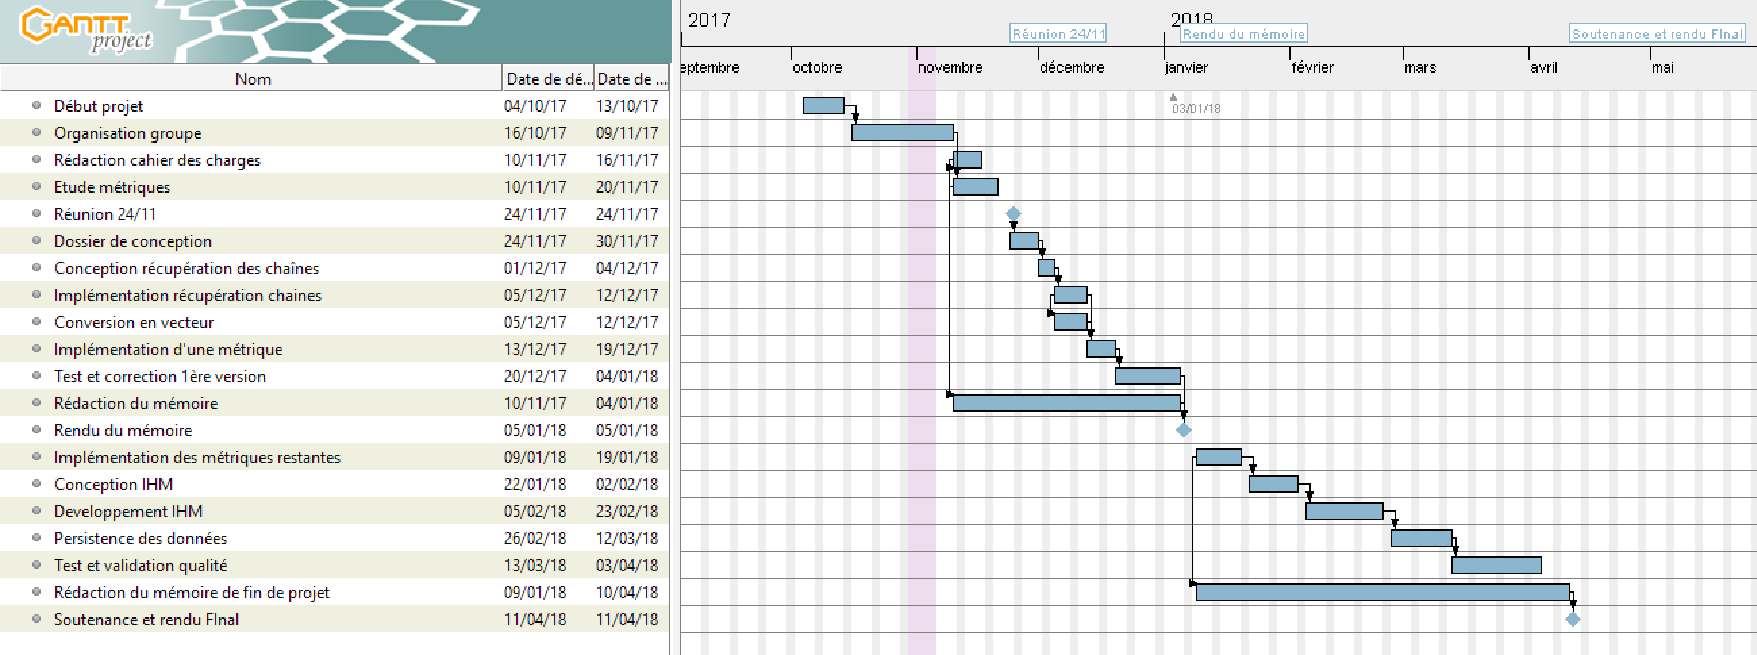
\includegraphics[scale=0.40]{gantt(1).pdf}}
  \caption{Diagramme de Gantt}
\end{figure}
\newpage
\subsection{Diagramme de PERT}
\begin{figure}[h]
  \centering{
  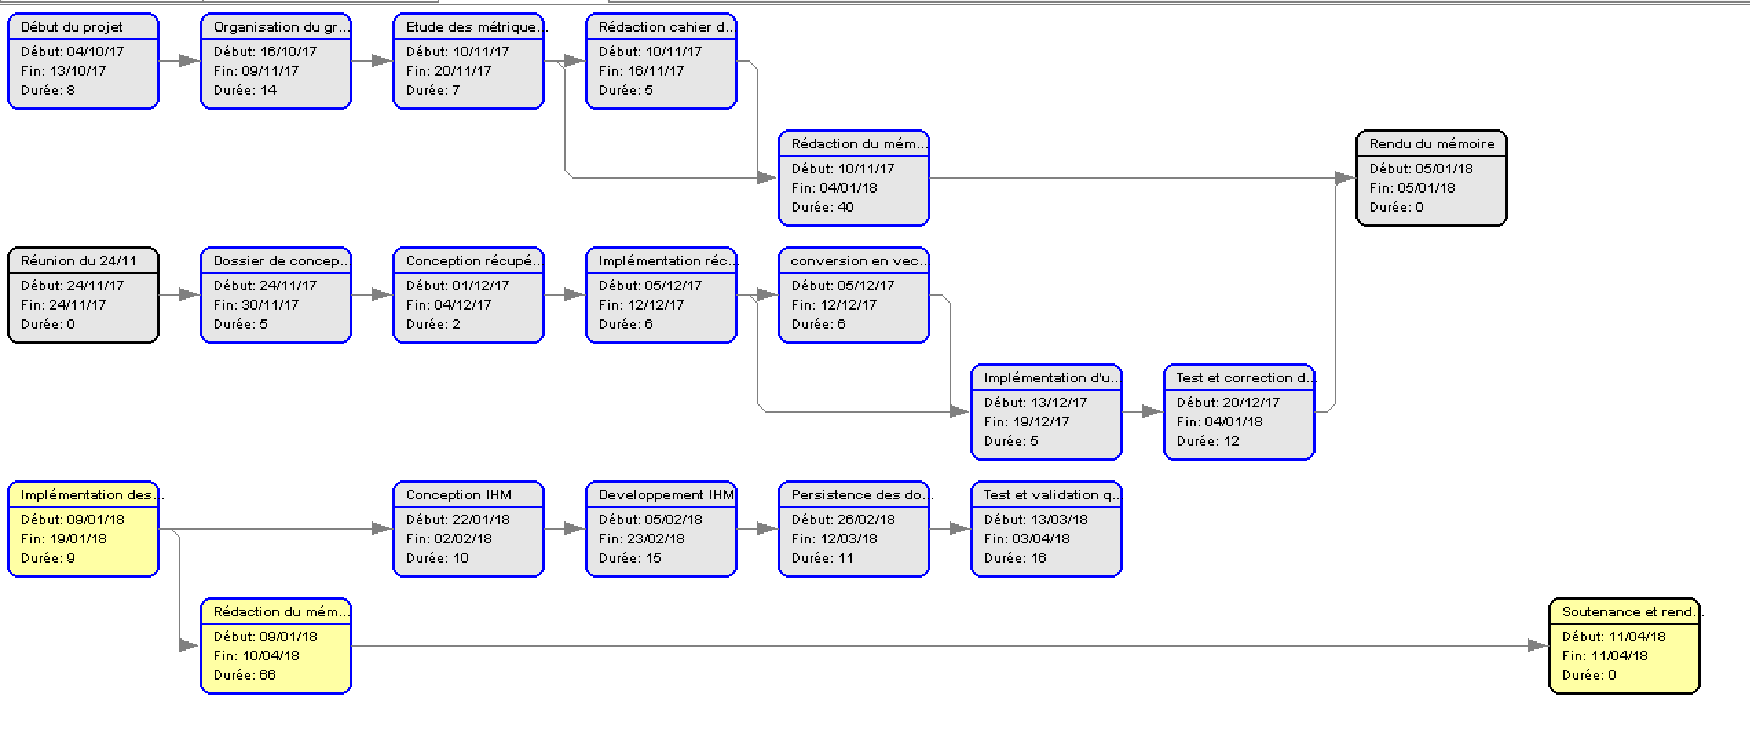
\includegraphics[scale=0.40]{pert(1)(1).pdf}}
  \caption{Diagramme de PERT}
\end{figure}



\subsection{Contexte}
Cette application est lié au mémoire de la première année de Master Informatique à l'université de Limoges. Le sujet du mémoire étant "Analyse forensic d'un Ransomware", cette application à pour objectif de déduire la classe d'un ransomware depuis une capture de mémoire vive d'un système infecté.

\subsection{Intérêts du document}
Ce document a pour but d'indiquer l'architecture et les choix techniques de l'application au développeur. Il indique ainsi toutes les informations nécessaires à la conception et au développement du programme. 

\subsection{Présentation de l'application}
L'application permettre à l'utilisateur de soumettre ces captures de mémoires à l'analyse, celle-ci lui renverra les taux de ressemblance de sa capture avec les différentes classes de ransomwares.
L'application est développée en langage Java.

\section{Description de l'application}
\subsection{Objectifs}
L'objectif de l'application est de permettre à l'utilisateur de pouvoir analyser au mieux les captures mémoires de ransomwares afin que celui-ci puisse en déduire facilement à quelles familles ils appartiennent. Pour cela, l'utilisateur aura accès à huit métriques différentes qui lui donneront huit différentes formes de rapprochements avec les classes de ransomwares.

Lors du lancement du programme, l'utilisateur indiquera le chemin 
du fichier à analyser et sélectionnera les métriques à utiliser.

Une fois l'analyse lancé, les résultats s'afficheront sous forme de tableau avec pour chaque métrique et classe de ransomware le rapprochement calculé.

\subsection{Architecture global de l'application}
L'architecture global de l'application se base sur un modèle standard MVC (Modèle Vue Contrôleur) de développement d'application et d'interface graphique.
\begin{figure}[!h]
\centering{
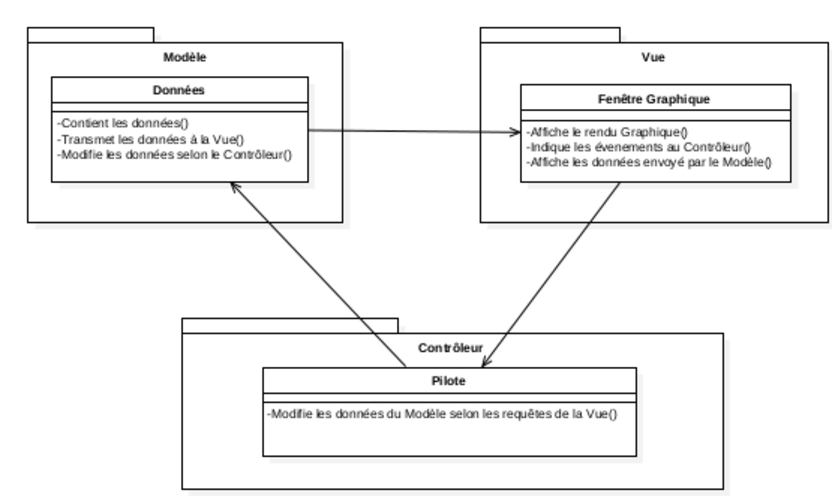
\includegraphics{MVC.pdf}}
\caption{Modèle MVC}
\end{figure}

\section{Conception}
\subsection{Architecture interne}
L'application est structurée de la maniére suivante :

\begin{figure}[!h]
\centering{
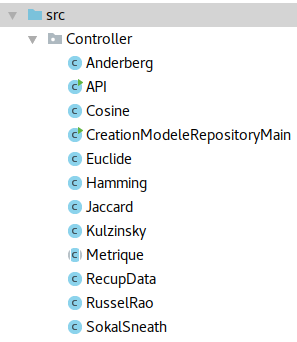
\includegraphics[scale=0.75]{controller.png}}
\caption{}
\end{figure}

\newpage
\begin{figure}[!h]
\centering{
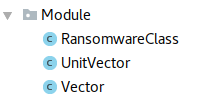
\includegraphics{modele.png}}
\caption{}
\end{figure}
\begin{figure}[!h]
\centering{

\includegraphics{vue.png}}
\caption{}
\end{figure}


\subsection{Algorithmes}

\section{Spécification des Données Persistantes}
\subsection{Données des classes de Ransomware}

\section{Spécification IHM}
\subsection{Schéma de Navigation}

Notre outil est extrêmement simpliste d'utilisation  :
\begin{figure}[!h]
\centering{
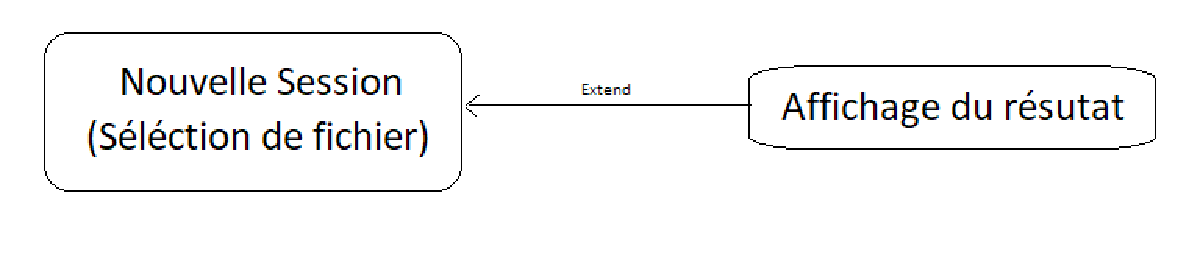
\includegraphics[scale=0.75]{utilisation.pdf}}
\caption{}
\end{figure}






\newpage
\subsection{Maquettes et Interface}
\begin{figure}[!h]
\centering{
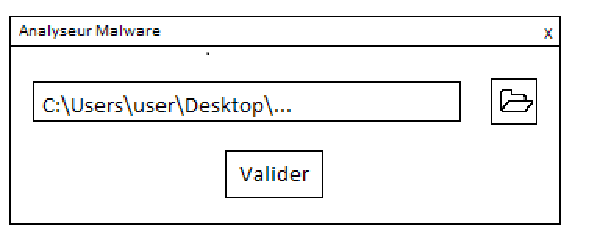
\includegraphics{maquette1.pdf}}
\caption{}
\end{figure}
\begin{figure}[!h]
\centering{
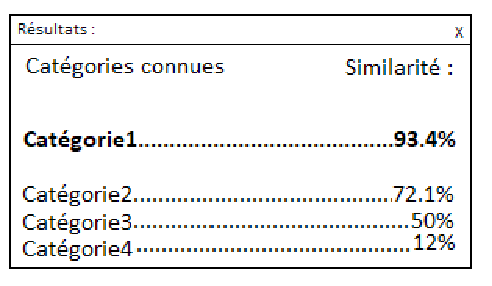
\includegraphics{maquette2.pdf}}
\caption{}
\end{figure}


L'interface utilisateur du programme se voudra relativement simpliste, le but de celle-ci sera avant tout d'être fonctionnelle plus que visuelle. 
Elle disposera d'une zone de saisie pour le chemin du fichier de capture qui sera l'entrée de notre programme, ainsi qu'un simple bouton pour lancer le balayage parmi la base de données(Figure2).

~\par
Une fois le balayage effectuée, une fenêtre s'ouvrira affichant le pourcentage de similarité entre l'entrée et les catégories les plus probable(Figure3). 
Autre possibilité : un bouton permettant d'afficher la base de données collectées jusqu'à présent par le programme.

\section{Qualité et complexité cyclique de l'application}
Le prototype a été implémenter en utilisant les services d'analyses de code du framework Intellj et de l'utilitaire Sonar ce qui permet d'avoir un code propre,suivant une nomenclature identique et commenté Les commentaires permettant de générer la documentation java.
La complexité cyclique a été calculé avec l'utilitaire MetricsReloaded et est actuellement de 1.68 ce qui est acceptable mais devra être amélioré au cours du second semestre.

\section{Objectifs du second semestre}
Au cours du second semestre nous allons améliorer le prototype afin qu'il devienne une application optimisée et puisse être utilisé dans les meilleures conditions pour faire de l'analyse forensic.
L'ergonomie et l'aspect visuel de l'application devront être améliorés afin que l'utilisateur puisse utiliser l'application de la manière la plus efficace possible et qu'il est directement accès à des résultats clairs et exploitables. L'utilisateur aura la possibilité de faire analyser plusieurs fichiers en même temps et consultera les résultats sur des graphiques clairs et concis.
Actuellement les fichiers utilisés sont déjà nettoyés, on souhaite que l'utilisateur est juste à nous soumettre des fichiers de capture mémoire brut afin d'obtenir des résultats il faudra donc créer un extracteur de chaînes.

L'utilisateur pourra sélectionner les métriques qu'il souhaite utiliser.
La quantité de famille de ransomware sera plus grande et les dictionnaires vectoriels (modèles et familles) seront améliorés afin qu'ils correspondent mieux aux métriques afin d'obtenir les meilleurs résultats possibles.

L'application devra ainsi être de la meilleure qualité possible afin de pouvoir la présenter lors de la soutenance de fin. d'année
\section{Conclusion}
Ce sujet nous permettra d'étudier le fonctionnement des ransomwares et leurs spécificités. Ce projet aboutira sur une application capable de classer les ransomwares ce qui sera une manière concrète de montrer nos connaissances et notre implication au cours de ce semestre.




\end{document}